\documentclass[12pt, psamsfonts]{amsart}

%-------Packages---------
\usepackage{amssymb,amsfonts}
\usepackage{fullpage}
\usepackage{todonotes}
\usepackage{physics}
\usepackage[all,arc]{xy}
\usepackage{enumerate}
\usepackage{mathrsfs}
\usepackage{theoremref}
\usepackage{graphicx}
\usepackage[bookmarks]{hyperref}

%--------Theorem Environments--------
%theoremstyle{plain} --- default
\newtheorem{thm}{Theorem}[section]
\newtheorem{cor}[thm]{Corollary}
\newtheorem{prop}[thm]{Proposition}
\newtheorem{lem}[thm]{Lemma}
\newtheorem{conj}[thm]{Conjecture}
\newtheorem{quest}[thm]{Question}

\theoremstyle{definition}
\newtheorem{defn}[thm]{Definition}
\newtheorem{defns}[thm]{Definitions}
\newtheorem{con}[thm]{Construction}
\newtheorem{exmp}[thm]{Example}
\newtheorem{exmps}[thm]{Examples}
\newtheorem{notn}[thm]{Notation}
\newtheorem{notns}[thm]{Notations}
\newtheorem{addm}[thm]{Addendum}
\newtheorem*{exer}{Exercise}

\theoremstyle{remark}
\newtheorem{rem}[thm]{Remark}
\newtheorem{rems}[thm]{Remarks}
\newtheorem{warn}[thm]{Warning}
\newtheorem{sch}[thm]{Scholium}

\DeclareMathOperator{\Hom}{Hom}
\DeclareMathOperator{\Id}{Id}

\makeatletter
\let\c@equation\c@thm
\makeatother
\numberwithin{equation}{section}

\bibliographystyle{plain}

\begin{document}

\title{Math 611 (Due 10/2)}
\author{Hidenori Shinohara}
\maketitle

\begin{exer}{(Problem 10, Chapter 1.3)}
  Find all the connected 2-sheeted and 3-sheeted covering spaces of $S^1 \vee S^1$, up to isomorphisms of covering spaces without base points.
\end{exer}

\begin{proof}
  \todo[inline]{
    For the first part, I ended up with the two graphs in Figure \ref{fig:problem10_idea}.
    Based on these three things, it's not hard to get to the following two possibilities.
    However, I'm not sure if this is rigorous enough.
    Also, I don't know how this can be applied to the case of 3.
    There are many ways to connect vertices and it doesn't seem doable, which suggests that there might be better ways to solve this.

    I tried to use the universal covering and consider a subset.
    I feel that this would make sure that I'm covering all the cases, although I don't know how to show it rigorously.
  }
  \begin{itemize}
    \item
      There have to be exactly two points in a covering space with 4 edges.
    \item
      Every other point has a neighborhood such that the point has only two edges.
    \item
      A covering space has to be path connected.
  \end{itemize}
 \begin{figure}
   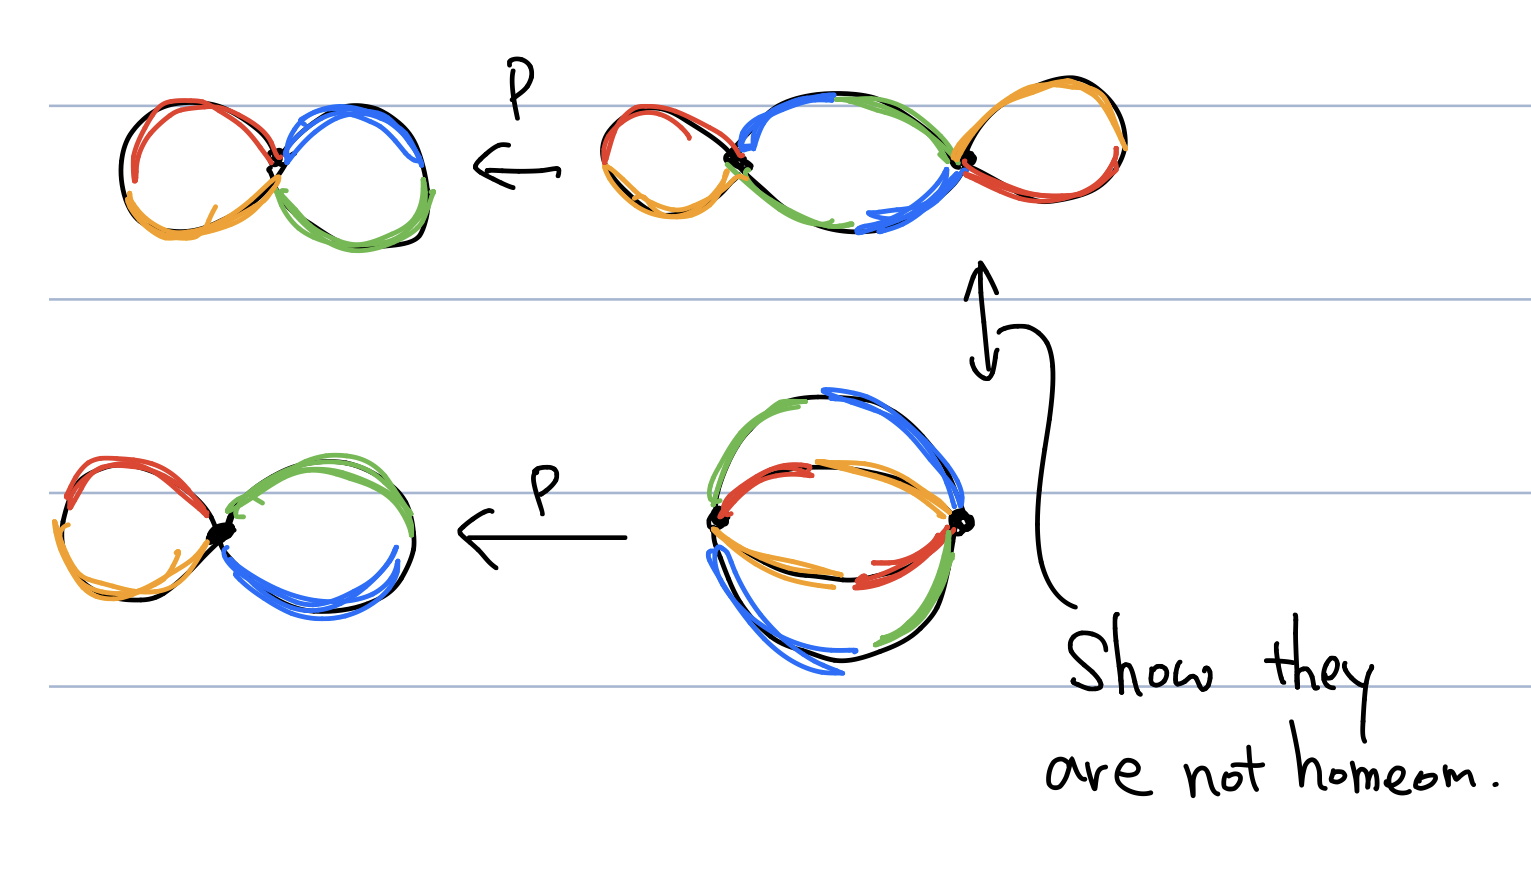
\includegraphics[width=.5\linewidth]{problem10_idea.jpeg}
   \caption{Problem 10 Idea}
   \label{fig:problem10_idea}
 \end{figure}
 \begin{figure}
   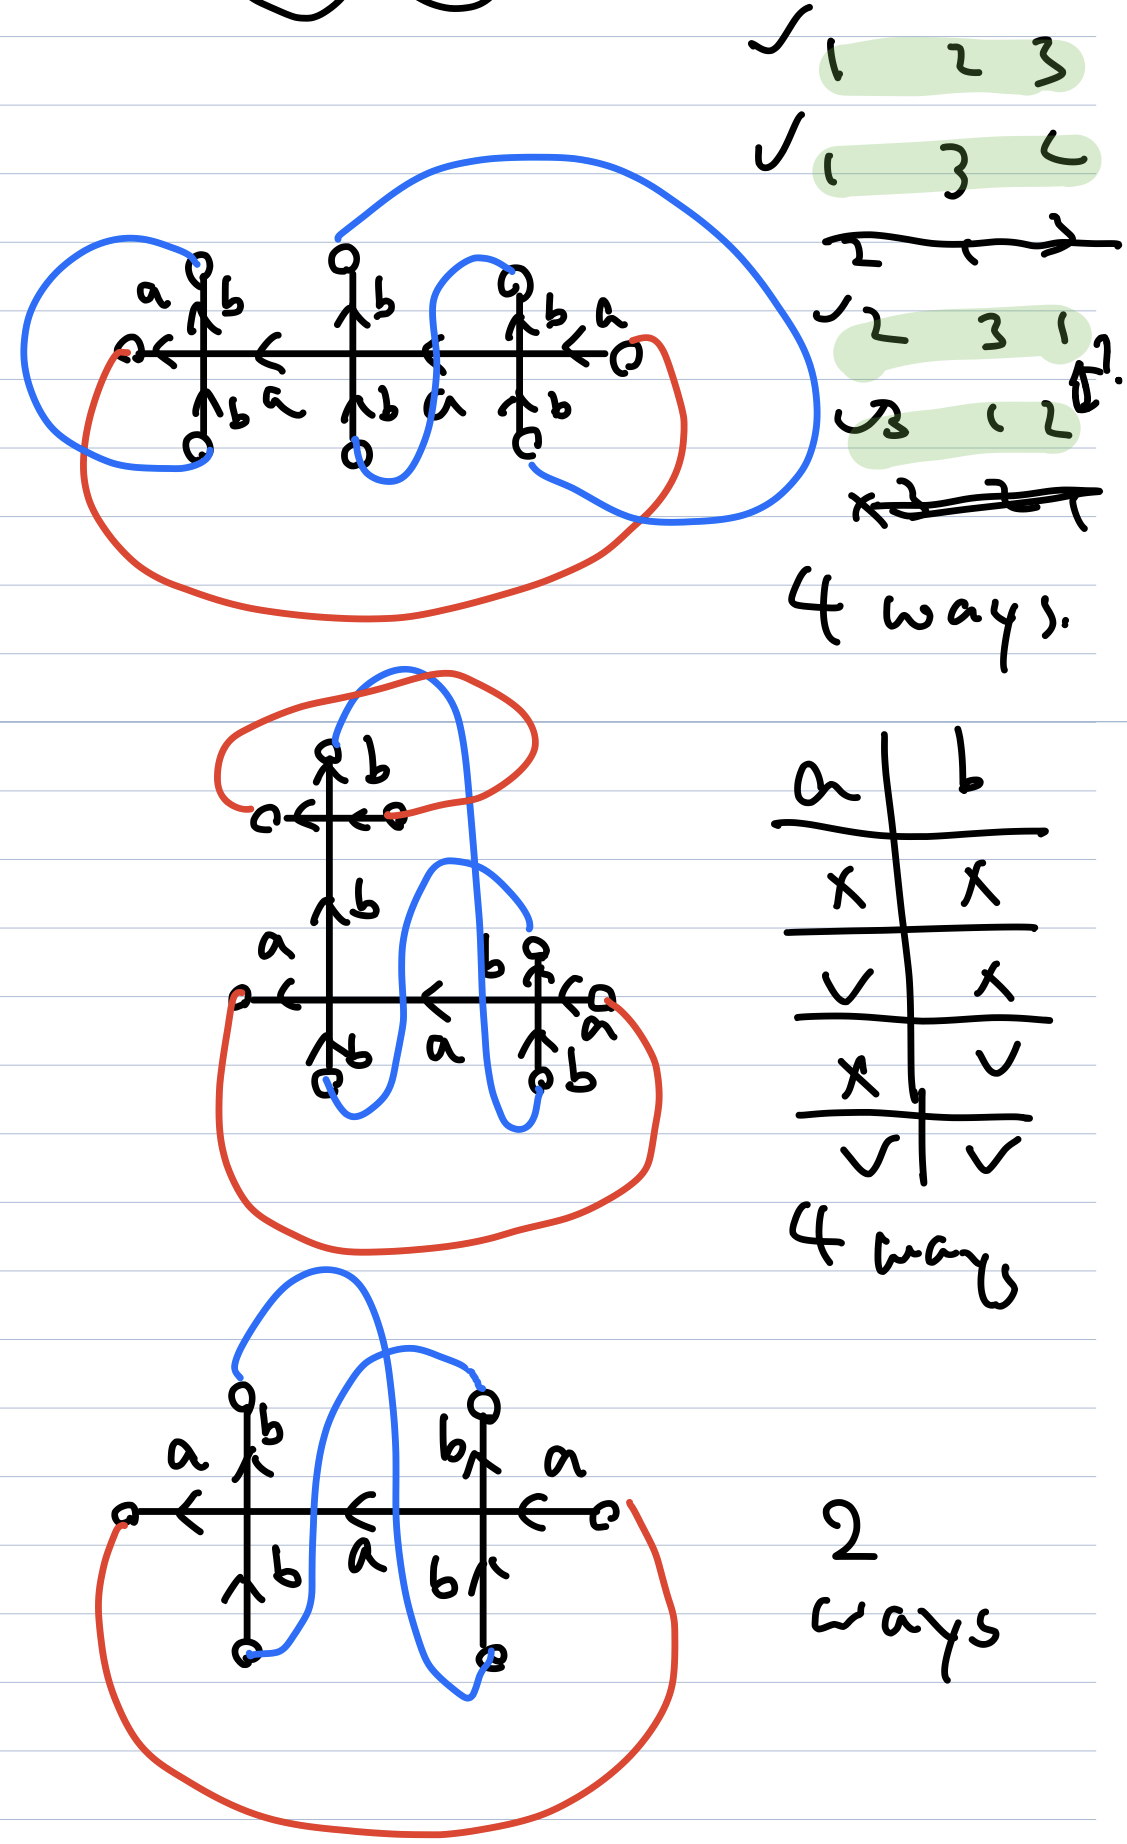
\includegraphics[width=.5\linewidth]{problem10_idea_2.jpeg}
   \caption{Problem 10 Idea 2}
   \label{fig:problem10_idea_2}
 \end{figure}
\end{proof}

\begin{exer}{(Problem 11, Chapter 1.3)}
  Construct finite graphs $X_1$ and $X_2$ having a common finite-sheeted covering space $\tilde{X}_1 = \tilde{X}_2$, but such that there is no space having both $X_1$ and $X_2$ as covering spaces.
\end{exer}

\begin{proof}
  Figure \ref{fig:problem11} shows $X_1, X_2$ and $\tilde{X}_1 = \tilde{X}_2$.
  \begin{figure}
    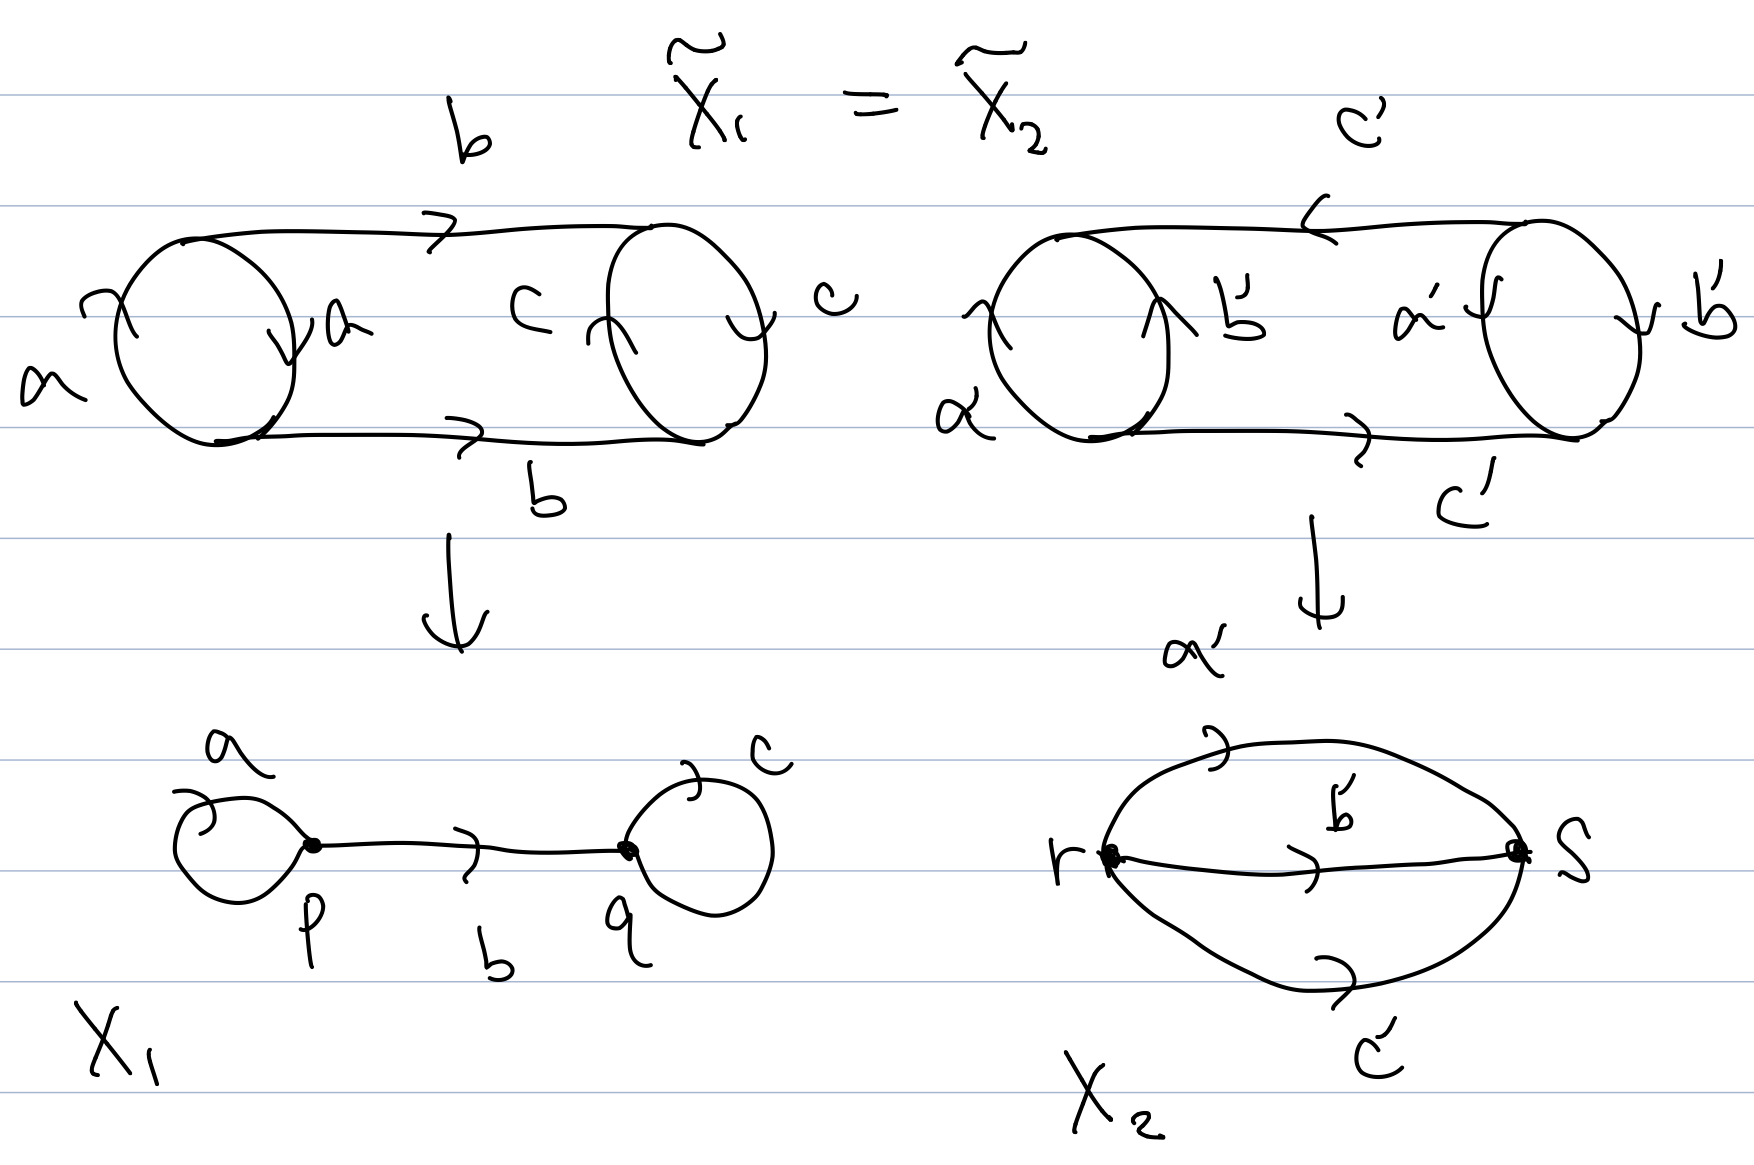
\includegraphics[width=.5\linewidth]{problem11.jpeg}
    \caption{Problem 11}
    \label{fig:problem11}
  \end{figure}
  
  We claim that there exists no space having both $X_1$ and $X_2$ as covering spaces.
  On the contrary, suppose there exists such a space $X$ with covering maps $p_1: X_1 \rightarrow X, p_2: X_2 \rightarrow X$.
  Then every point in $X$ must have a neighborhood that homeomorphic to an open subset of $X_1$.
  Since $X_1$ is a graph, that means $X$ is locally a line and a vertex with edges.
  In other words, $X$ must be a graph.

  There must exist a neighborhood of $p_1(p)$ and a neighborhood of $p$ such that they are homeomorphic.
  Since $p$ is a vertex of degree 3, $p_1(p)$ must be a vertex of degree 3 as well.
  Similarly, $p_1(q)$ must be a vertex of degree 3 as well.

  Since $p, q$ are the only vertices of $X_1$, $X$ contains at most two vertices and their degrees must be 3.
  Since the sum of degrees of all vertices must be even from elementary graph theory, $X$ must contain two vertices of degree 3.

  If $X$ only consists of loops, then the degree of each vertex will be even.
  Thus the two vertices must be joined by at least one edge.
  Then if one vertex has a loop, the other must have a loop as well in order to have degree 3.
  If there exists another edge joining the two vertices, there must be a third one in order for the two vertices to have degree 3.
  Therefore, $X_1, X_2$ are the only graphs with two vertices of degree 3.

  Suppose that $X_1$ is a covering space of $X_2$ with a covering map $f: X_1 \rightarrow X_2$.
  Without loss of generality, $f(p) = r, f(q) = s$.
  Consider the path $a'$ in $X_2$.
  Lifting $a'$ to $X_1$ will result in a path from $p$ to $q$.
  This implies that $f$ maps points on the path $b$ into points on a path $a'$.
  
  Now consider the path $b'$ in $X_2$.
  Lifting $b'$ to $X_1$ will again result in a path from $p$ to $q$.
  This implies that $f$ maps points on the path $b$ into points on a path $b'$.

  This implies that every point on the path $b$ must be mapped to $r$ or $s$.
  This is a contradiction because $f$ is continuous and $\{ b(t) \mid t \in [0, 1] \}$ is connected, but $\{ r, s \}$ is disconnected.

  Thus $X_1$ is not a covering space of $X_2$.

  Similarly, suppose that $X_2$ is a covering space of $X_1$ with a covering map $g: X_2 \rightarrow X_1$.
  Without loss of generality, $g(r) = p, g(s) = q$.
  This implies $g^{-1}(p) = \{ r \}$, so the number of sheets is 1.
  In other words, $g$ is injective.
  Consider the path $a$ in $X_1$.
  Lifting $a$ to $X_2$ results into a loop based at $r$.
  Since $a: I \rightarrow X_1$ is injective, $\tilde{a}: I \rightarrow X_2$ is injective since $g \circ \tilde{a} = a$.
  Then $\tilde{a}(t) = s$ for some $t \in [0, 1]$, so $a(t) = g(\tilde{a}(t)) = g(s) = q$.
  However, $q$ is not a point on $a$.
  This is a contradiction, so $X_2$ is not a covering space of $X_1$.

  Hence, there exists no space that has both $X_1$ and $X_2$ as covering spaces.
\end{proof}

\begin{exer}{(Problem 14, Chapter 1.3)}
  Find all the connected covering spaces of $\mathbb{R}P^2 \vee \mathbb{R}P^2$.
\end{exer}

\begin{proof}
  \todo[inline]{
    I think Figure \ref{fig:problem14_idea_2} is the universal covering of $\mathbb{P}_2 \wedge \mathbb{P}_2$, but I'm not certain.
  }
  \begin{figure}
    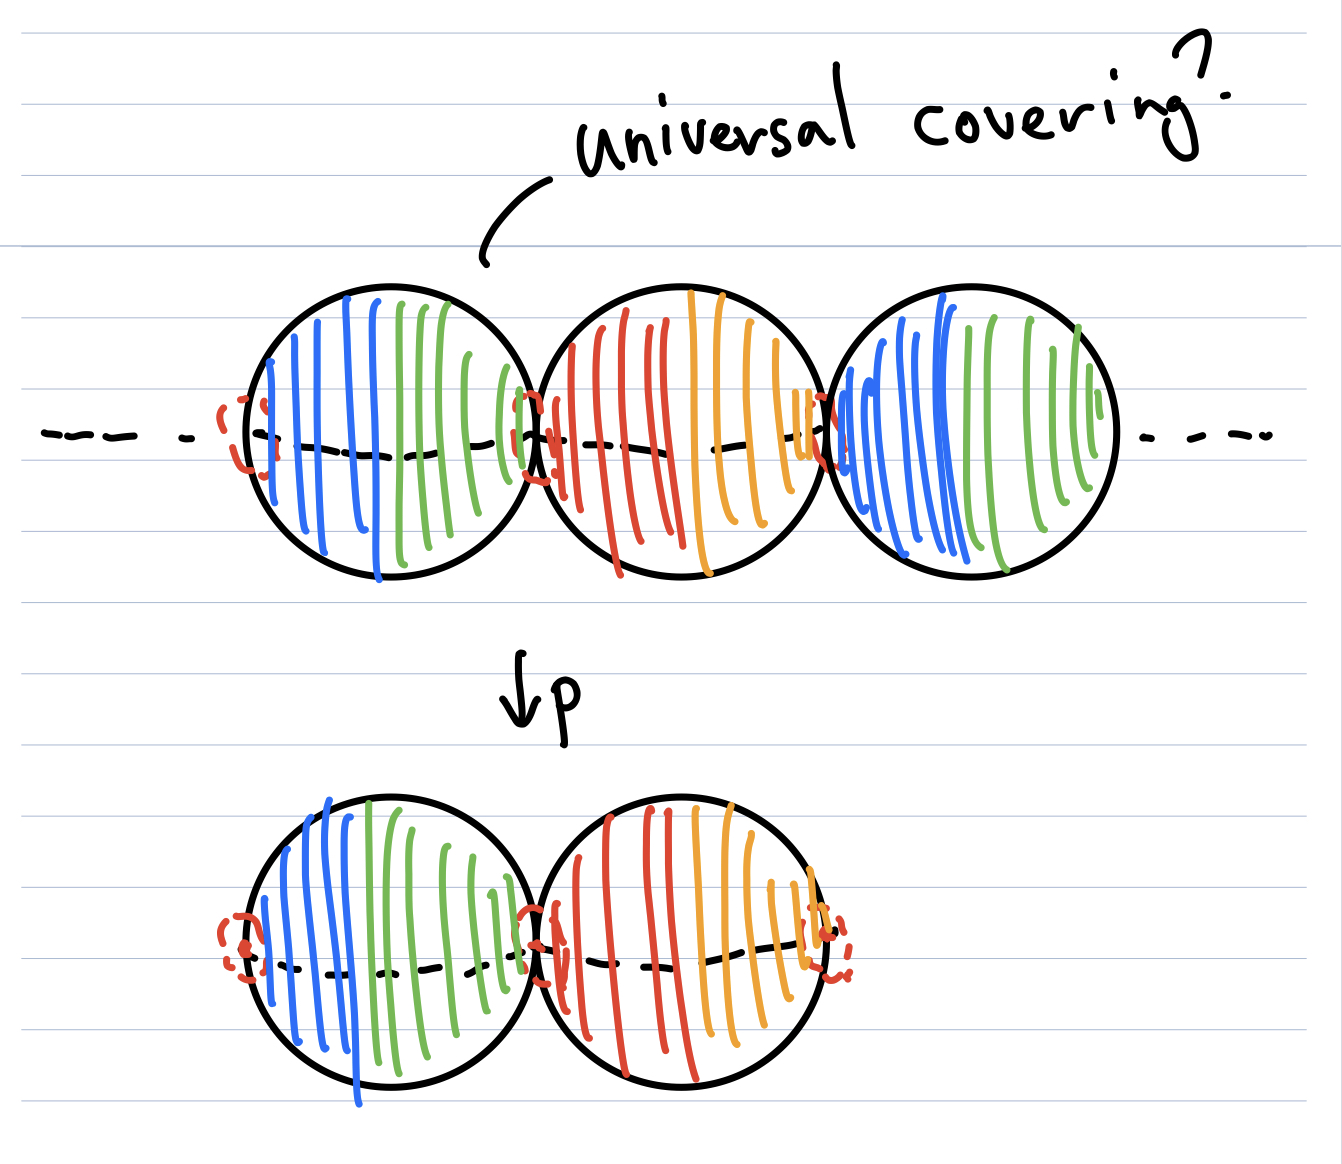
\includegraphics[width=.5\linewidth]{problem14_idea_2.jpeg}
    \caption{Problem 14 Idea 2}
    \label{fig:problem14_idea_2}
  \end{figure}
\end{proof}

\end{document}


